\section{Optimization Methods}

In this section I will present a few optimization algorithms.

\subsection{Line Search Methods}

The {\color{tiananmen}\textbf{line search}} is a strategy that selects the step size (commonly represented by $t$) that determines where along the line $\left\lbrace x+t\Delta x\mid t\in\mathbb{R}_+\right\rbrace$ the next iterate in the descent method will be. ($\Delta x$ represents the \textit{descent direction}, .) Line search strategies can either be \textit{exact} or \textit{inexact}.

\subsubsection*{Exact Line Search}

An {\color{tiananmen}\textbf{exact line search}} chooses the value $t$ along the ray $\left\lbrace x+t\Delta x\mid t\in\mathbb{R}_+\right\rbrace$ that exactly minimizes the function of interest $f$:
{\color{baystate}$$t=\arg\min_{s\geq 0}f(x+s\Delta x)$$}
An exact line search is almost never practical. In very special cases, such as some quadratic optimization problems, where computing the cost of the minimization problem is low compared to actually calculating the search direction, one might employ an exact line search.

\subsubsection*{Backtracking Line Search}
Most often in practice we use {\color{tiananmen}\textbf{inexact line searches}}. In an inexact line search, we choose $t$ such that $f$ is \textit{approximately} minimized or reduced ``enough'' along $\left\lbrace x+t\Delta x\mid t\in\mathbb{R}_+\right\rbrace$.

One inexact line search strategy is the {\color{tiananmen}\textbf{Backtracking Line Search}}.
\begin{algorithm}[H]
	\caption{Backtracking Line Search \cite[]{Boyd2004}\label{BacktrackingLineSearchAlg}}
	\begin{algorithmic} 
		\State \textbf{given} a descent direction $\Delta x$ for $f$ at $x\in\textbf{dom}f,\alpha\in(0,0.5),\beta\in(0,1)$.
		\State $t:=1$.
		\While{$f(x+t\Delta x)>f(x)+\alpha t\nabla f(x)^T\Delta x$}
		\State $t:=\beta t$
		\EndWhile
	\end{algorithmic}
\end{algorithm}

``Backtracking'' in the name is refers to the fact that the method starts with a unit step size $(t=1)$ and then reduces the step size (``backtracks'') by the factor $\beta$ until we meet the stopping criterion $f(x+t\Delta x)\leq f(x)+\alpha t\nabla f(x)^T\Delta x$.

%%% Need to reproduce image on own or something for final draft...

Figure 9.1 \cite[p. 465]{Boyd2004} demonstrates the Backtracking Line Search visually for a parabola.
\begin{center}
	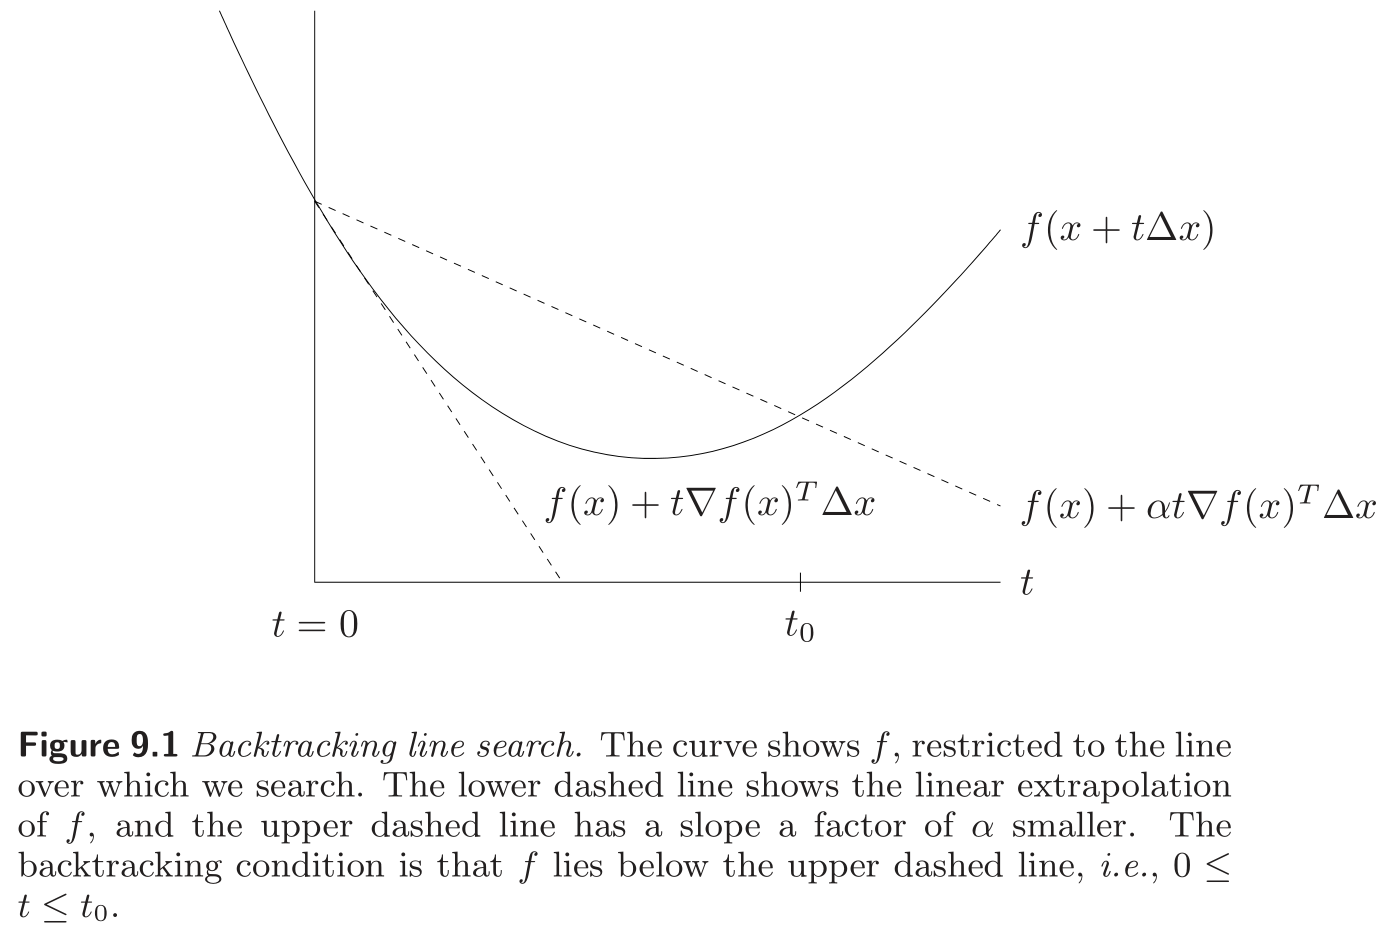
\includegraphics[width=0.75\textwidth]{Chapter_I_Background/Images/backtracking_line_search_diagram.png}
\end{center}

Notice that the backtracking search will find a step size $t$ such that $0\leq t\leq t_0$ and that for such $t$, $f(x+t\Delta x)$ is smaller relative to $f(x)$. However, the step size we choose may not exactly be the minimum of the function, but we have funneled it down to be closer to the minimum of $f$.
\subsection{Gradient Descent}

\subsection{Conjugate Gradient}